\documentclass[11pt,a4paper]{article}
        \usepackage[margin=20mm]{geometry}
        \usepackage[T1]{fontenc}
        \usepackage{lmodern}
        \usepackage{amsmath,amssymb,graphicx,booktabs,float,array,caption}
        \usepackage[hidelinks]{hyperref}
        \setlength{\parindent}{0pt}
        \setlength{\parskip}{5pt}
        \setlength{\tabcolsep}{5pt}
        \emergencystretch=2em
        \renewcommand{\arraystretch}{1.12}
        \captionsetup{font=small,labelfont=bf}
        \begin{document}

\begin{center}{\LARGE\bfseries Look Ahead Car Following Control}\\[5pt]

{\large INTR 5100 \quad Lab Session II}\\[5pt]Group 4 \quad HKUST(GZ) \quad Fall 2026\end{center}

\subsection*{Overview}

We compare predictive PID, LQI and MPC using one recorded Group 4 run per method and previously saved simulations. The MPC-labelled run follows at smaller gaps under a shorter target policy. PID has lower student-to-middle speed variation ratios in the two excited nonlaunch events. LQI closes a large inherited gap. These observations show different spacing and disturbance responses without establishing an overall controller ranking.


\section*{1 Experiment setup and data preparation}

The SC2I testbed uses a prescribed-speed leader, an IDM-controlled middle vehicle and a student-controlled follower. The student callback receives all three states and their histories, then returns a desired speed command. Steering and the lower-level speed response remain in the supplied program. Student control operates only when middle and student share a selected straight; bypass intervals use the supplied logic.


\begin{table}[H]\centering\small\caption{Recorded experimental configuration}
\begin{tabular}{ll}
\toprule
Setting & Value \\
\midrule

Geometry & Vehicle length 250 cu; route loop 15,700.81 cu \\

Middle IDM & v0 70; T 1.2; s0 250; a 20; b 30; exponent 4 \\

Timing & Configured 0.15 s; observed decisions about 0.20 s \\

Student spacing shield & PID 80 cu; MPC and LQI 50 cu \\

Physical data & One 2.8-labelled run per method; same role identifiers \\

\bottomrule\end{tabular}\end{table}

The earlier Group 1 deployment-error run is excluded. Initial gaps and predecessor histories differ across the retained runs. Source hashes and MPC solver status were not logged during physical testing; method names identify the recorded runs, rather than proving which internal control mode produced every command.


\subsection*{Event processing}

Consecutive student\_straight decisions define four events, matched by selected-section index and occurrence: 3, 1, 2, 3. The three trajectories are aligned on a 0.1 s grid without extrapolation; source interpolation spans above 0.3 s are rejected. Middle and student must share the same selected section. Event 1 includes launch; event 4 is quiet and ends with the recording.


Spacing is forward route distance minus 250 cu. Position jumps and some approximately 0.5 s telemetry gaps limit differentiated acceleration, jerk and TTC. Coordinate units are retained because physical scale and command-response gain remain unresolved.


\newpage

\section*{2 Controller design}

\subsection*{Speed conventions and target policies}

Let q be reported speed, v coordinate speed and u the returned command. Telemetry conversion gamma and command response beta are distinct hypotheses. The 2.8 variants set both to 2.8; this does not establish either as a measured platform constant. Position-derived speeds already use cu/s and receive no additional factor.


\[
v=\gamma q,\qquad u=v_{\rm desired}/\beta,\qquad \gamma=\beta=2.8
\]

\begin{table}[H]\centering\small\caption{Own target bumper gaps in the 2.8 variants}
\begin{tabular}{lrr}
\toprule
Method & Target gap in cu & At q = 40 \\
\midrule

PID and LQI & 300 + 1.8v & 501.6 cu \\

MPC & 250 + 1.2v & 384.4 cu \\

\bottomrule\end{tabular}\end{table}

MPC therefore seeks a gap 117.2 cu shorter at reported speed 40. Own-target error evaluates each policy and cannot by itself rank all methods against a common spacing objective.


\subsection*{Predictive PID and LQI}

PID estimates leader acceleration from recent history and uses a 0.8 s rollout of the supplied middle IDM logic with an assumed 0.5 s response lag. It blends current and forecast middle speed, then adds spacing feedback. The middle command memory is approximated; forecast accuracy is limited by gating, sensor stops and vehicle response.


\[
e=s-(300+1.8v),\qquad r=0.55v_M+0.45\widehat v_M(t+0.8)
\]

\[
u_{\rm nominal}=(r+0.12e+0.002I+0.08D)/\beta
\]

I is accumulated spacing error and D its filtered derivative. Anti-windup, inactive-interval resets, stale-state checks, command limits and closing protection modify the nominal command. LQI uses the same target and forecast with normalized spacing, relative-speed and integral states. Its discrete Riccati feedback uses Q = diag(4, 2, 1) and unit control penalty. These designs and gains are retained unchanged.


\subsection*{MPC and implementation limits}

MPC uses 12 steps of 0.2 s, history-based predecessor trends and an assumed 0.5 s lag. Its objective penalizes gap error, speed deviations and command changes, subject to speed, rate and predicted-gap constraints. Optimization requires NumPy, CVXPY and OSQP; otherwise its feedback fallback may operate. Physical logs do not distinguish that fallback from successful optimization.


\newpage

\section*{3 Recorded results and analysis}

\subsection*{3.1 Active control and spacing errors}

\begin{table}[H]\centering\small\caption{Student command-log overview during active control}
\begin{tabular}{lrrrrr}
\toprule
Run & Active / total & Min gap & Median gap & Spacing flags & Sensor flags \\
\midrule

PID & 337 / 768 & 92.3 & 385.4 & 0 & 2 \\

MPC & 368 / 785 & 103.2 & 293.9 & 0 & 0 \\

LQI & 362 / 801 & 105.6 & 425.7 & 0 & 0 \\

\bottomrule\end{tabular}\end{table}

Gaps are in cu and flag counts are command rows, not independent incidents. All active gaps exceed a common 80-cu band. PID has two consecutive active sensor-flag rows; MPC and LQI each have one sensor flag during bypass. No active spacing shield or wrapper fallback is recorded. Sensor-event causes and MPC internal fallback status remain unverified.


\begin{table}[H]\centering\small\caption{Aligned trajectory samples and own-target spacing errors}
\begin{tabular}{lrrrrr}
\toprule
Event & Run & Samples & Entry to exit gap & RMSE & Bias \\
\midrule

1 & PID & 281 & 116.4 to 411.4 & 114.5 & -84.2 \\

1 & MPC & 275 & 103.2 to 315.6 & 94.9 & -84.1 \\

1 & LQI & 328 & 113.9 to 458.1 & 107.5 & -45.6 \\

2 & PID & 81 & 241.4 to 387.2 & 157.3 & -147.6 \\

2 & MPC & 114 & 146.9 to 262.2 & 175.2 & -170.2 \\

2 & LQI & 100 & 291.6 to 438.5 & 137.0 & -119.8 \\

3 & PID & 202 & 518.6 to 477.1 & 57.2 & 46.1 \\

3 & MPC & 211 & 372.6 to 379.4 & 37.4 & 30.2 \\

3 & LQI & 188 & 664.6 to 463.6 & 131.6 & 102.3 \\

4 & PID & 77 & 414.0 to 455.5 & 55.6 & -54.0 \\

4 & MPC & 91 & 305.6 to 342.1 & 52.0 & -50.3 \\

4 & LQI & 93 & 401.1 to 468.3 & 61.3 & -57.5 \\

\bottomrule\end{tabular}\end{table}

RMSE is the square root of mean squared gap error; bias is mean gap minus target. Both use retained aligned samples and cu. Positive bias denotes a gap above the method's target. These event metrics differ from command-log summaries because their sampling and synchronization masks differ.


Event 2 begins below target for every method, with different entry gaps. In event 3, LQI removes about 201 cu of separation, PID about 42 cu, while MPC approximately maintains its smaller gap. LQI's large inherited gap contributes to its higher RMSE. A common-route restriction preserves this interpretation without equalizing initial states or disturbance histories.


\newpage

\subsection*{3.2 Trajectories and disturbance propagation}

\begin{figure}[H]\centering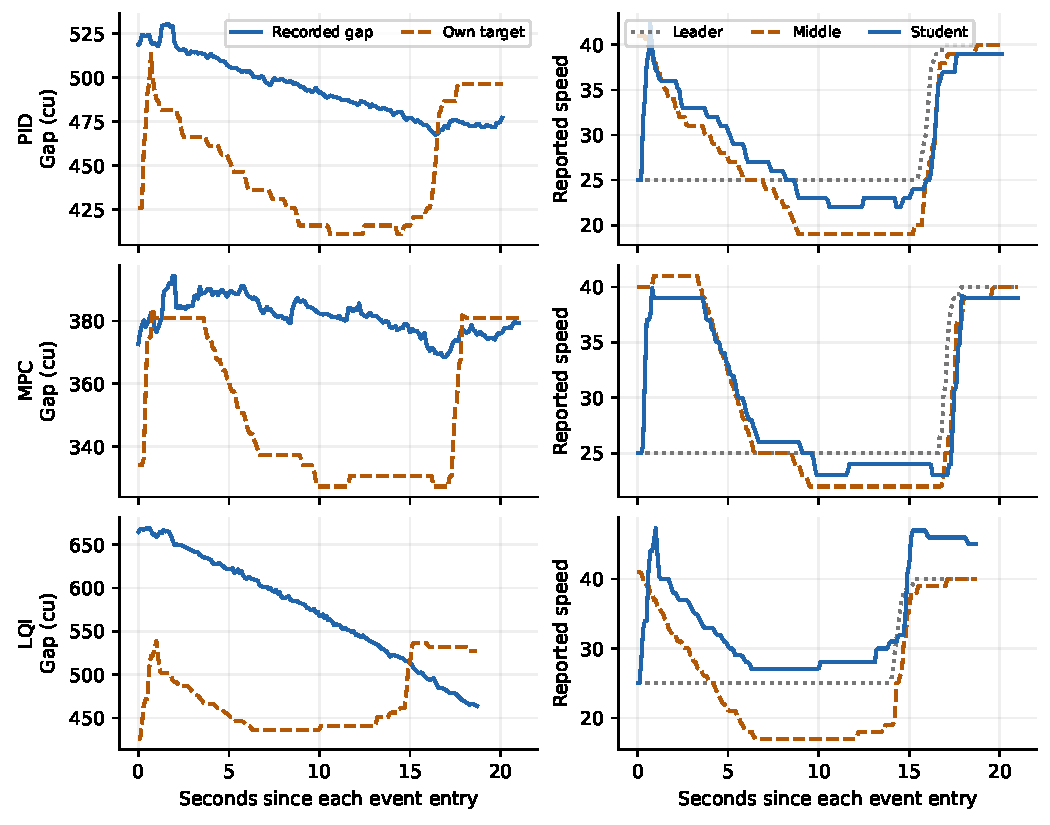
\includegraphics[width=\linewidth]{figures/event_3_records.pdf}\caption{Event 3 recorded gaps, own targets and all three reported speeds. Each row starts at its own event entry; elapsed time does not represent matched disturbances across runs.}\end{figure}

\begin{table}[H]\centering\small\caption{Demeaned reported-speed standard deviation ratios}
\begin{tabular}{lrrrr}
\toprule
Event & Run & Middle / leader & Student / middle & Student / leader \\
\midrule

2 & PID & 0.696 & 0.866 & 0.603 \\

2 & MPC & 0.488 & 1.010 & 0.493 \\

2 & LQI & 0.715 & 1.002 & 0.716 \\

3 & PID & 1.368 & 0.776 & 1.061 \\

3 & MPC & 1.395 & 0.834 & 1.163 \\

3 & LQI & 1.508 & 0.795 & 1.199 \\

\bottomrule\end{tabular}\end{table}

Ratios use the same retained samples within each event; a common constant speed conversion cancels. PID has the smallest student/middle ratio in events 2 and 3. In event 3 all methods attenuate middle-speed variation, yet student/leader remains above one, so upstream amplification is not fully removed. Event 4 has zero middle-speed variation and no meaningful ratio.


These finite-window observations do not prove string stability. The formation has only three vehicles, unequal inputs and switched protections; frequency-dependent amplification and longer-platoon behavior are not established [1].


\newpage

\subsection*{3.3 Previously saved simulation evidence}

The following numbers come from the existing analysis records. No response model was refitted and no simulation was repeated for this revision. These supplementary results are kept separate from the physical measurements.


\subsection*{Recorded command response model}

The saved first-order plant fit used rounded commands and one-second route-displacement residuals, with alternating 5 s training and validation blocks. This is validation within one recording, rather than on an independent experimental run. The gain absorbs unresolved scale and dynamics.


\begin{table}[H]\centering\small\caption{Saved held-out one-second displacement errors}
\begin{tabular}{lrrrrr}
\toprule
Input run & Gain & Lag s & Delay s & RMSE cu & Relative RMSE \\
\midrule

PID & 2.914 & 0.10 & 0.00 & 17.87 & 16.7\% \\

MPC & 2.937 & 0.10 & 0.10 & 17.64 & 16.5\% \\

LQI & 2.973 & 0.80 & 0.00 & 16.46 & 15.8\% \\

\bottomrule\end{tabular}\end{table}

Relative RMSE divides by mean held-out displacement. PID and MPC select the lowest tested lag, 0.10 s, indicating weak identification or omitted dynamics. The differing fits for the same student vehicle and 15.8-16.7\% errors limit the model's predictive authority.


\subsection*{Student feedback with recorded predecessors}

In the saved study, each controller drove a simulated student using recorded leader and middle trajectories. Student position and speed evolved from commands after initialization; recorded student states were reference data. Front vehicles remained externally imposed. Assumptions included the 2.8 telemetry scale, source-specific plant fit, actual decision times, bypass gating and nominal obstacle inputs.


\begin{table}[H]\centering\small\caption{Saved baseline own-target gap RMSE in cu}
\begin{tabular}{lrrr}
\toprule
Recorded front input & PID & MPC & LQI \\
\midrule

PID & 137.8 & 79.5 & 146.0 \\

MPC & 113.0 & 69.4 & 119.9 \\

LQI & 120.5 & 71.0 & 133.8 \\

\bottomrule\end{tabular}\end{table}

Nine baseline cases plus half/double-lag variants total 27 saved simulations. They record no sampled negative gap, spacing-shield activation or callback exception. Some MPC decisions are protective stops, so even the simulated MPC cases are not optimization-only trajectories. These sampled outcomes provide conditional evidence, not a collision-avoidance guarantee.


MPC has the lowest baseline own-target RMSE under this model. Different target policies and approximately 79-121 cu same-method simulated-versus-recorded position RMSE prevent translating that ranking into demonstrated physical superiority.


\newpage

\subsection*{3.4 Efficiency comfort and safety}

\subsection*{Local spacing and flow}

For moving samples with reported speed at least 5, use v = 2.8q, bumper time gap s/v, reciprocal space occupancy 1000/(s + 250), and local flow proxy v/(s + 250). The latter quantities describe one pair's local spacing and motion; they are not measured detector flow, network density or road capacity.


\begin{table}[H]\centering\small\caption{Median kinematic proxies under the 2.8 speed hypothesis}
\begin{tabular}{lrrrr}
\toprule
Event & Run & Time gap s & Vehicles / 1000 cu & Flow proxy veh/s \\
\midrule

2 & PID & 3.71 & 1.67 & 0.158 \\

2 & MPC & 1.78 & 2.16 & 0.252 \\

2 & LQI & 3.97 & 1.60 & 0.152 \\

3 & PID & 6.60 & 1.35 & 0.101 \\

3 & MPC & 5.24 & 1.58 & 0.115 \\

3 & LQI & 6.86 & 1.21 & 0.104 \\

\bottomrule\end{tabular}\end{table}

MPC has higher local flow proxies in these events, consistent with its shorter gap policy. Inherited separation also affects the values. These data cannot isolate an algorithmic improvement in network throughput, and unresolved metric scale prevents conversion to vehicles/km.


\subsection*{Comfort and timing}

The RMS sent-command increments are PID 1.48, MPC 1.50 and LQI 1.46 command units. They use consecutive active decisions excluding flagged pairs. These small differences describe command activity, not measured acceleration, jerk or ride comfort. Localization steps and speed quantization make a physical comfort ranking unreliable.


The approximately 0.20 s decision interval is loop cadence, not end-to-end response latency. Previously saved local callback benchmarks exclude communication and actuator delay and do not establish physical timing performance.


\subsection*{Safety and energy}

Observed active minimum gaps are 92.3, 103.2 and 105.6 cu for PID, MPC and LQI. None activates the recorded spacing shield, although native thresholds differ. Unequal launch gaps, unverified sensor causes and limited repetition prevent a safety ranking or a general collision-avoidance claim. TTC would additionally depend on validated speed, timing and closing-sign conventions.


No fuel flow, electrical power or calibrated energy model is recorded. Fuel consumption, Wh/km and percentage energy savings therefore cannot be established. The earlier positive-kinetic-variation diagnostic measures repeated speed increases and excludes road load, efficiency and regeneration; it is not a fuel result.


\newpage

\section*{4 Discussion and conclusions}

\subsection*{What the look ahead information contributes}

An upstream leader can reveal a disturbance before it fully appears in the middle vehicle's speed. The known middle IDM gives PID and LQI a basis for anticipating that response; MPC uses predecessor trends. Feedforward can therefore complement immediate spacing feedback, as motivated by cooperative-control studies [1-3]. Hidden command memory, asynchronous telemetry, safety overrides and response lag still limit prediction.


Earlier slowing can reduce a later speed transient while enlarging the gap temporarily. Feedback must subsequently recover that separation. This explains why spacing accuracy and attenuation can trade off, but the physical tests do not isolate this mechanism: every candidate uses look-ahead information, MPC has a shorter policy, and there is no matched physical controller using only the immediate predecessor.


\subsection*{Conclusions supported by the records}

The MPC-labelled run maintains the smallest gaps under its chosen policy. PID shows the lowest student/middle reported-speed variation ratios in the two excited nonlaunch events. LQI recovers substantially from its larger event-3 entry gap. All three retain positive recorded active gaps, with no active spacing-shield flags. The records support these scenario-specific observations and do not select one method across tracking, safety, comfort, stability and energy.


Any future causal comparison would need common targets, initial conditions and disturbances, repeated runs and explicit optimizer-status logging. A matched look-ahead ablation would separate the contribution of upstream information from controller tuning. Those are limits of the current evidence; the completed experiments and saved results are retained here without replacement.


\subsection*{References}

[1] G. J. L. Naus et al. Cooperative adaptive cruise control, design and experiments. American Control Conference, 2010, pp. 6145-6150. DOI: 10.1109/ACC.2010.5531596.


[2] C. Wang et al. Cooperative adaptive cruise control for connected autonomous vehicles by factoring communication-related constraints. Transportation Research Part C 113, 2020, pp. 124-145. DOI: 10.1016/j.trc.2019.04.010.


[3] C. Wu, Y. Lin and A. Eskandarian. Cooperative Adaptive Cruise Control With Adaptive Kalman Filter Subject to Temporary Communication Loss. IEEE Access, 2019. DOI: 10.1109/ACCESS.2019.2928004.


\subsection*{Experimental record}

Sources are the Lab II guidelines, supplied experiment/controller files, the three Group 4 raw-run folders, and saved physical\_summary.json, event CSVs, macro\_metrics.json and closed\_loop.json in results/three\_controller\_analysis. The earlier deployment-error record is retained separately. Controller code and original data/results are unchanged; report tables use recorded observations or explicitly identified historical simulations.


\end{document}